\chapter{INTRODUCTION} \label{intro}

The fundamental structure of the universe has remained an enduring fascination of mankind. The philosophers of antiquity speculated that the world could be decomposed into the base elements of water, earth, fire, and air. The alchemists of the Middle Ages, regarding the classical elements to be expressions of hidden substance, sought to unveil its nature with crude experiments. The scholars of the Renaissance rejected the Aristotelian description of physical phenomena for its empirical failures and pondered if atoms were the indivisible units of matter. The chemists of the 19th century advanced and refined the atomic theory in their pursuit to catalog the pure elements. The physicists of the 20th century realized the necessity of a quantum description of the universe while delving into the subatomic realm. The scientific paradigm of the current era now rests on the theoretical framework known as the Standard Model of particle physics which, though understood to be incomplete, has had its predictions verified with remarkable accuracy.

\section{The Standard Model}

The fundamental forces\footnote{Gravity, which does not have a satisfactory quantum description, falls outside of the Standard Model.} and forms of matter within the universe are explained by the Standard Model in terms of elementary particles, their antiparticles, and their interactions. The following subsections highlight the features of the model necessary to motivate the treatise of this paper. A formal and rigorous treatment of the theory is beyond the scope of this paper but may be found in such texts as Ref. \cite{Peskin} and \cite{Schwartz}.

The Standard Model is a relativistic quantum field theory (QFT) in which fundamental particles are understood to be excitations of their associated fields that permeate all of space-time. The fundamental forces are generated by the internal gauge symmetry of the model \symSM, which give rise to the strong (\symSTRONG), weak (\symWEAK), and electromagnetic (\symEM) interactions. Its current formulation is thus a combination of electroweak theory with quantum chromodynamics (QCD). The particles manifested by the model may be broadly categorized into \textit{fermions} and \textit{bosons} and a visual summary is shown in Figure \ref{fig:SM}.

\begin{figure}[htbp]
  \centering
    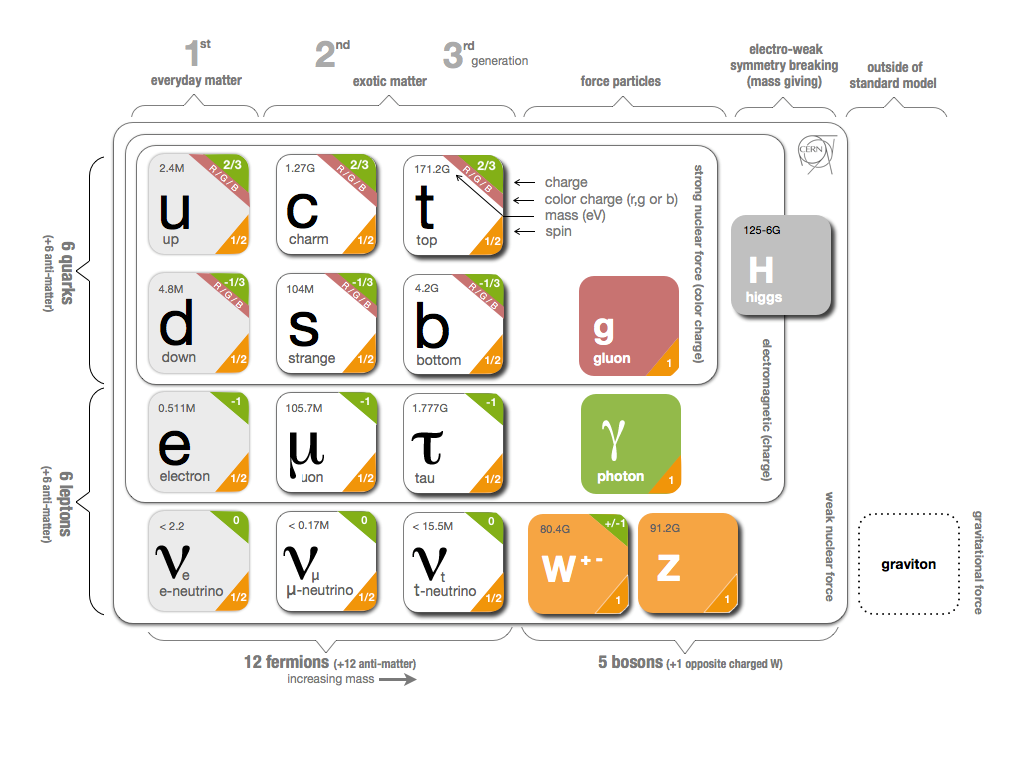
\includegraphics[width=6in]{images/SMinfographic_image}
    \caption[Standard Model Infographic]{An infographic of the Standard Model. The elementary particles are arranged in their usual generational pairs and the surrounding solid lines divide them into sections based on the fundamental forces they experience.\cite{Purcell:1473657}}
    \label{fig:SM}
\end{figure}

\subsection{Fermions}

The fermions encompass all forms of ordinary and exotic matter and obey Fermi-Dirac statistics because of their half-integer spin, namely, spin-\ensuremath{\frac{1}{2}}. They are divided into \textit{leptons} and \textit{quarks}. The electrically charged leptons interact via the electromagnetic and weak nuclear forces and include the familiar \textit{electron} (\lepe), the \textit{muon} (\lepm), and the \textit{tau} (\lept). The charged leptons also have neutral counterparts (\lepne, \lepnm, \lepnt) known as \textit{neutrinos}, which interact solely via the weak nuclear force. The quarks, having both electric and color charge, interact via the electromagnetic and strong and weak nuclear forces and include the up (\qrku), down (\qrkd), charm (\qrkc), strange (\qrks), bottom (\qrkb), and top (\qrkt). Although the leptons can exist freely, the nature of the strong interaction gives rise to color confinement, whereby quarks only appear within composite particles called hadrons. The bound states of quark doublets are known as mesons while those of quark triplets, of which the familiar proton is an example, are known as baryons.

The leptons and quarks are each arranged into pairs by flavour quantum number and sorted into three generations of increasing mass\footnote{The observation of neutrino oscillations disproved the prediction that they are massless but its implications for the lepton generations are unclear.}, as depicted in Figure \ref{fig:SM}. The more massive particles of the higher generations decay into the stable particles of the first generation, which corroborates the observation that ordinary matter consists of electrons and up and down quarks which are bound in protons and neutrons. There are no known constraints on the number of fermion generations, although experimental results suggest there are only three.

\subsection{Bosons}

The bosons, which obey Bose-Einstein statistics because of their integer spin, are divided into vector and scalar bosons. The spin-1 vector, or gauge, bosons mediate the fundamental forces and are exchanged between elementary particles during their interactions. The photon \bosg\ mediates the electromagnetic force, which is responsible for the phenomenon of intermolecular repulsion.\footnote{It is this repulsion that prevents us from passing through objects.} The \bosW\ and \bosZ\ bosons mediate the weak nuclear force that causes nuclear decay. And finally, the gluons \bosgln\ mediate the strong nuclear force that binds quarks into hadrons and even protons and neutrons in nuclei. The only spin-0 scalar boson in the theory is the Higgs boson, which is responsible for the masses of the heavy gauge bosons and fermions.

\subsection{The Higgs Mechanism}

The requirement of gauge invariance under \symWEAK\ leads to a prediction of massless gauge bosons, which stands in contrast to the observation that the weak vector bosons are massive. In order to reconcile this observation while preserving the gauge invariance of the interaction, a mechanism of \textit{spontaneous symmetry breaking} was incorporated into the unified electroweak theory proposed by Sheldon Glashow \cite{EWKGLASHOW}, Abdus Salam \cite{EWKSALAM}, and Steven Weinberg \cite{EWKWEINBERG}. This mechanism, which came to be known as the \textit{Higgs mechanism}, was independently developed by Robert Brout and Fran\c{c}ois Englert \cite{HIGGSBE}, its namesake Peter Higgs \cite{HIGGSH}, and Gerald Guralnik, Richard Hagen, and Sir Thomas Kibble \cite{HIGGSGHK}.



\section{The Higgs Boson}

\subsection{Production Modes}

\subsection{Decay Modes}

\subsection{Discovery at the LHC}

Example citation of ATLAS Higgs discovery paper. \cite{ATLASHiggsDiscovery}

\section{Searches for \VHbb}

\subsection{Motivation for \VHbb}

\subsection{Results from Past Experiments}

\subsection{Results from the LHC}

%We don't make the Chapter titles in All Caps Automatically because it is easier for you to type your Chapter Titles in uppercase than for those that need to have mixed case in their titles to find the correct command in the ufthesis.cls file and change it there. \renewcommand*{\thefootnote}{\fnsymbol{footnote}}\footnote{an un-numbered footnote - this is how you tell the readers that this chapter was previously published and then cite the Journal where it was published} We don't recommend that you change much of anything in the class file unless you're absolutely sure of what your are doing.\renewcommand*{\thefootnote}{\arabic{footnote}}\setcounter{footnote}{0}\footnote{and now we're back to normal footnote marking} 


%Title case is where all principal words are capitalized except prepositions, articles, and conjunctions.  %\cite{green2008wrinkle}

%\subsection{Subsection Commands Are Also in Title Case}
%The difference, of course, are the second level headings are left-aligned
%
%\subsubsection{Subsubsections are in sentence case}
%The third level subheadings are left-aligned but in sentence case. Only the first letter and any proper nouns are capitalized. %\cite{strickler1998contamination}
%
%\subsubsection{If you divide a section, you must divide it into two, or more, parts}
%
%{\bf Paragraph headings.} There is no official fourth level heading. Do not use the Paragraph heading feature in LaTeX, simply apply the bold characteristic to the first few words of a paragraph followed by a colon or period.

%\subsection{I Need Another Second Level Heading in This Section}
%
%Aliquam mi nisi, tristique at rhoncus quis, consectetur non mi. Phasellus blandit quam ligula, a viverra lacus commodo at. In iaculis nisl vel pretium sollicitudin. In efficitur massa vel elit sollicitudin, vel auctor sapien cursus. Proin feugiat sapien a mi tempus;
%
% $ X-X'=D+D'$
%
% in consequat augue cursus. Nulla sed sagittis purus. Nunc eu consequat orci, eu laoreet enim. Ut euismod tincidunt sem, eget lacinia dui luctus eu. Aliquam mi augue, faucibus id semper vitae, porta ac ligula. Morbi sed ultrices odio. Mauris id luctus ex. Nulla ac libero dictum, interdum turpis lacinia, scelerisque leo. Praesent varius orci ac eros varius pharetra.
%
%\section{Image Handling in XeLaTeX}
%
%One of the biggest reasons for switching from the dvipdfm/dvipdfmx methods of compiling is the improved image handling capabilities. EPS, Bit-mapped, PDF, JPG, and PNG formats work well with the xelatex process.
%
%\subsection{The Traditional EPS Format}
%
%EPS format is the traditional format for LaTeX, but EPS files can be very large and many programs can't create or view these images. There are many programs that are used to interpret data and output the results as an EPS format image. It has been my experience that there are bounding box problems with these figures. On many occasions we have opened the image in Adobe Photoshop and, without making any changes, saved the document as a Photoshop EPS file, re-compiled the document, and the image worked correctly, so if you are having problems with an EPS image not showing in your document correctly, try this fix first.
%
%
%\begin{figure}[htbp]
%  \centering
%    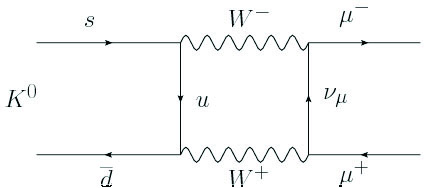
\includegraphics[width=5in]{images/diagram}
%    \caption[EPS format diagram. Note: no filetype is designated by adding an extension.]{EPS format diagram. Note: no filetype is designated by adding an extension. The file type is determined and the correct procedure is automatically chosen by xelatex.}
%\end{figure}
%
%
%Quisque malesuada a leo eget ullamcorper. Curabitur ut aliquam quam. Nam quis quam id mauris aliquam blandit porttitor sit amet quam. Donec ut erat eleifend turpis finibus pulvinar.
%
%\subsection{Bitmapped Images Work As Well}
%
%Bitmapped images are a standard file type on PCs, but these files are also usually very large so compressed images may be a better alternative.
%
%\begin{figure}[htbp]
%  \centering
%    \includegraphics[width=5in]{images/eagle}
%    \caption[BMP format drawing. Note: no filetype is designated by adding an extension.]{BMP format drawing. Note: no filetype is designated by adding an extension. The file type is determined and the correct procedure is automatically chosen by xelatex.}
%\end{figure}
%
%Morbi hendrerit risus nec quam posuere viverra. Donec quis tellus faucibus, molestie arcu sed, congue urna. Duis eget neque ac libero pulvinar porta eget et magna. Donec a magna eu eros suscipit cursus ac vitae nisl. Vivamus ligula purus, congue sed tortor blandit, ultrices egestas nisl.
%
%\subsection{Not to Mention PDF}
%
%It is often very handy to be able to include a pdf file as an image. By using XeLaTeX this is usually just matter of setting the size, or scale properties correctly.
%
%\begin{figure}[htbp]
%  \centering
%    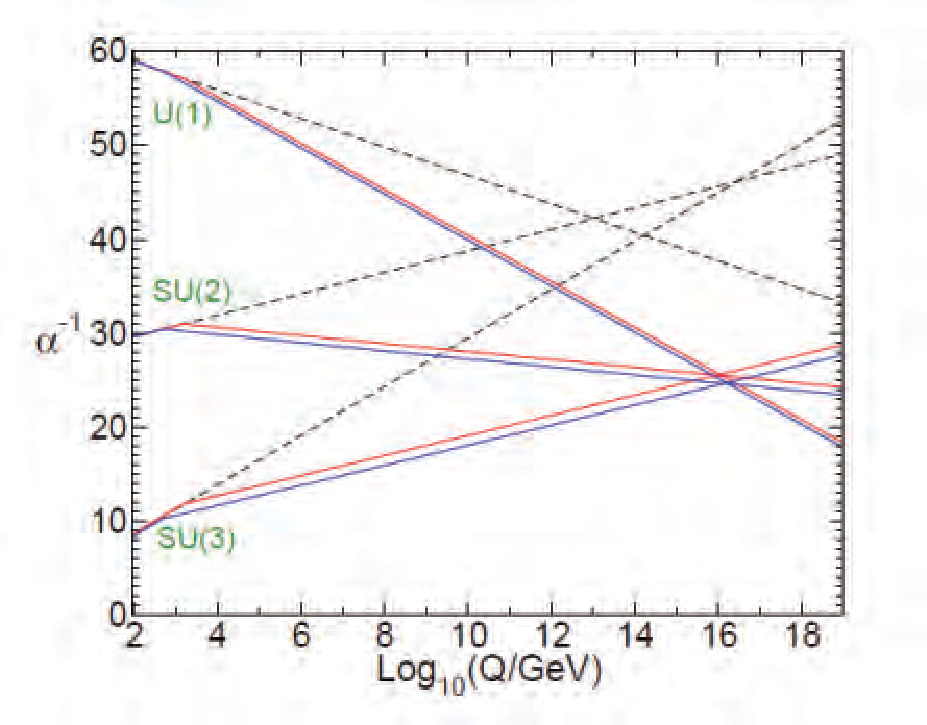
\includegraphics[scale=1.0]{images/graph.pdf}
%    \caption[PDF format graph. Note: no filetype is designated by adding an extension.]{PDF format graph. Note: no filetype is designated by adding an extension. The file type is determined and the correct procedure is automatically chosen by xelatex.}
%\end{figure}
%
%Nulla mattis augue lacus. Nam non lectus dolor. Cras ac quam vel justo elementum vestibulum. Integer vulputate pulvinar lacus sit amet pulvinar.
%
%\subsection{JPG Is Absolutely Necessary}
%
%For photographs, JPG is the most common format. This format is a fraction of the size of Bit-mapped images and can deliver very good quality at a much smaller overhead. Vestibulum eu lectus vel orci dictum vehicula. Proin id maximus dolor. Integer augue ante, pulvinar ac erat vitae, porttitor ullamcorper libero. %\cite{l2012wrinkle}
%
%\begin{figure}[htbp]
%  \centering
%    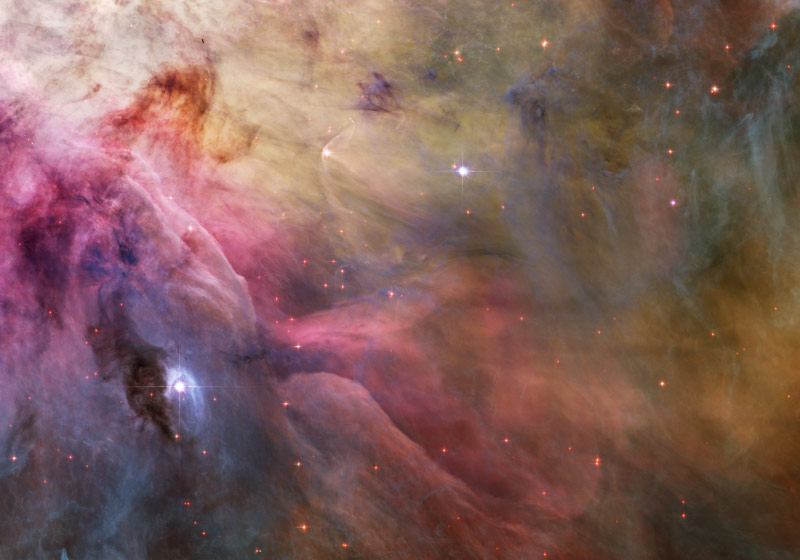
\includegraphics[width=5in]{images/nebula}
%    \caption[JPG format image. Note: no filetype is designated by adding an extension.]{JPG format image. Note: no filetype is designated by adding an extension. The file type is determined and the correct procedure is automatically chosen by xelatex.}
%\end{figure}
%
%Nunc blandit scelerisque velit, ac facilisis dui finibus et. Sed facilisis tortor vel commodo luctus. Donec est felis, malesuada id nibh in, accumsan malesuada lectus. Sed lobortis volutpat felis, vitae aliquet augue congue id. Fusce ut odio tincidunt, condimentum nulla vel, pharetra arcu.
%
%\subsection{PNGs Will Help Make Files Smaller}
%
%PNG files are even smaller than JPGs and are very good when text and images are combined.
%
%\begin{figure}[htbp]
%  \centering
%    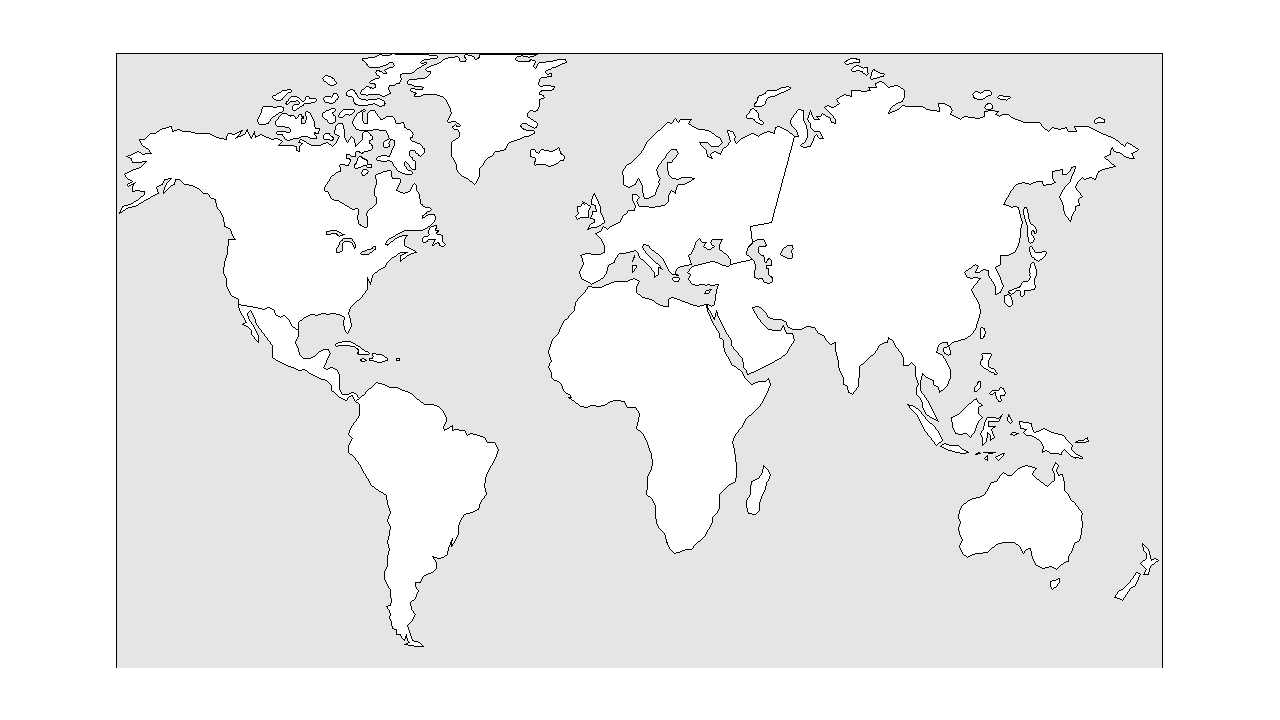
\includegraphics[width=5in]{images/theworld}
%    \caption[PNG format map. Note: no filetype is designated by adding an extension.]{PNG format map. Note: no filetype is designated by adding an extension. The file type is determined and the correct procedure is automatically chosen by xelatex.}
%\end{figure}
%
%
%
%Aenean condimentum libero sed mi porta, tempus ullamcorper lectus venenatis. Aliquam in diam dolor. Maecenas tempus consectetur sem et pulvinar. Aenean aliquam at metus ut hendrerit. Vivamus molestie ac neque eu luctus. Nam convallis maximus quam non lobortis. Fusce sit amet lorem et massa convallis aliquet at sit amet nulla. Suspendisse nec ex elit. Aenean gravida, sapien vitae congue commodo, urna turpis ornare libero, at cursus risus libero in erat. %\cite{Rust94}
%
%\section{GIF, TIF, and Others}
%
%Other file formats have not been successful, with or without file extensions. The tests have not been exhaustive so if you have a different type, give it a try. GIF, and TIF both do NOT work at this time. The next image demonstrates how to use multiple images as a single figure. Notice, there is a single caption for ALL figures and that caption starts with a discription of the ENTIRE figure before breaking off into the subfigure descriptions.
%
%\begin{figure}[htbp]
%     \centering
%   \mbox{
%      \subfigure [] {
\includegraphics[scale=0.6]{images/mouse}} \qquad
%      \subfigure []{
\includegraphics[scale=0.6]{images/mouse}} \qquad
%     }
%    \mbox{
%      \subfigure [] {
\includegraphics[scale=3]{images/cat}} \qquad
%      \subfigure [] {
\includegraphics[scale=0.6]{images/mouse}} \qquad
%      }
%    \caption[Tom and Jerry]{Tom and Jerries. This caption demonstrates how the sub-captions are left out of the List of Figures, but included in the figure itself. A) Tom the first; B) Tom the second; C) Jerry; D) Tom the third.}
%    \label{mice}
%  \end{figure}
%
%
%Aliquam mi nisi, tristique at rhoncus quis, consectetur non mi. Phasellus blandit quam ligula, a viverra lacus commodo at. In iaculis nisl vel pretium sollicitudin. In efficitur massa vel elit sollicitudin, vel auctor sapien cursus. Proin feugiat sapien a mi tempus, in consequat augue cursus. Nulla sed sagittis purus. Nunc eu consequat orci, eu laoreet enim. Ut euismod tincidunt sem, eget lacinia dui luctus eu. Aliquam mi augue, faucibus id semper vitae, porta ac ligula. Morbi sed ultrices odio. Mauris id luctus ex. Nulla ac libero dictum, interdum turpis lacinia, scelerisque leo. Praesent varius orci ac eros varius pharetra.
%
%
%
%Nunc blandit scelerisque velit, ac facilisis dui finibus et. Sed facilisis tortor vel commodo luctus. Donec est felis, malesuada id nibh in, accumsan malesuada lectus.
%\begin{itemize} %
%    \item WinEDT: This text editor is recommended for use editing \TeX-files as it has many useful built in macros and is easy to use  %
%    \item This program can be found and downloaded here: \url{http://www.winedt.com/} %
%    \item The GIMP (GNU Image Manipulation Program) %
%    \begin{itemize}%
%        \item A freeware graphics editing program for picture editing and file conversions %\vspace{-12pt}%
%        \item Comparable to Adobe Photoshop %\vspace{-12pt}%
%        \item Can be downloaded here: \url{http://www.gimp.org/}%
%    \end{itemize}
%    \item A good reference of \LaTeX 2\ensuremath{\epsilon} commands%
%    \begin{itemize}
%        \item This should be included on the ETD website here: \url{http://etd.helpdesk.ufl.edu/tex.php}
%    \end{itemize}
%\end{itemize} %
%
%
%Sed lobortis volutpat felis, vitae aliquet augue congue id. Fusce ut odio tincidunt, condimentum nulla vel, pharetra arcu. In ultricies libero diam, nec rutrum magna vehicula nec. Praesent dictum eros sit amet turpis ultricies, eleifend condimentum dui imperdiet. Donec congue urna ante, id rutrum mi commodo a. Vivamus id tincidunt nunc. Morbi id lacus ut augue ultricies convallis. Duis a lectus quis ante pretium scelerisque nec nec nisi. In id porta justo, at euismod diam. Suspendisse vel tempus arcu. Praesent vel cursus nisi, ac rhoncus odio.

